\begin{figure}[htbp]
	\centering
	\resizebox{\textwidth}{!}{%
		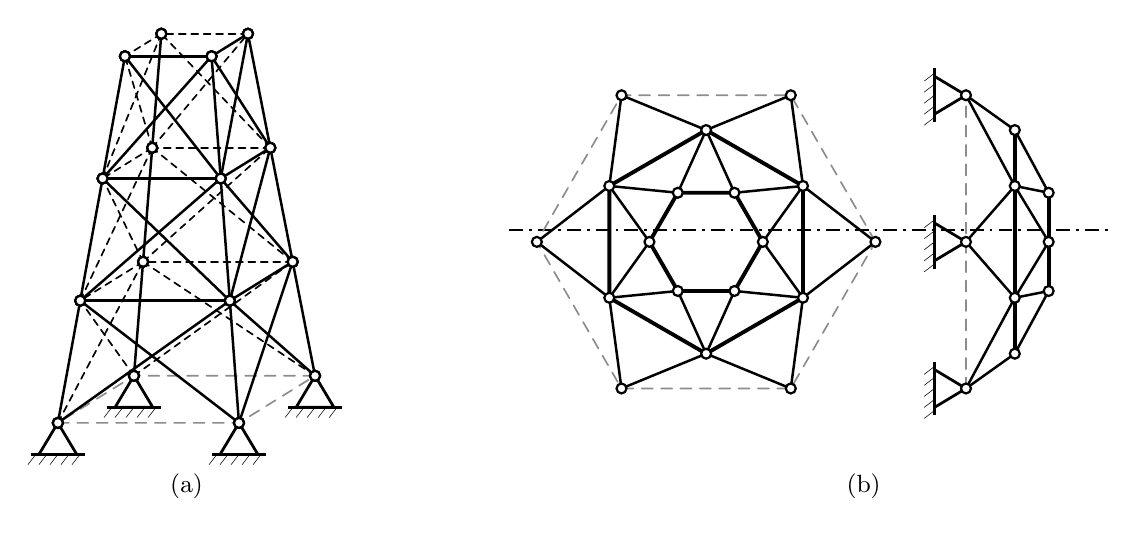
\begin{tikzpicture}[
			asta/.style={line width=0.9pt, line cap=round, line join=round, black},
			anello/.style={line width=1.4pt, line cap=round, line join=round, black},
			anellobase/.style={line width=0.6pt, line cap=round, black!45,	dash pattern=on 4pt off 3pt},
			nascosta/.style={line width=0.6pt, line cap=round, black,dash pattern=on 2.5pt off 2pt},
			assesim/.style={line width=0.6pt,dash pattern=on 5pt off 2.2pt on 1pt off 2.2pt},
			nodo/.style={circle, fill=white, draw=black, inner sep=0pt, minimum size=4.5pt, line width=0.9pt},
			nodino/.style={circle, fill=white, draw=black,	inner sep=0pt, minimum size=3.6pt, line width=0.8pt},
			etich/.style={font=\small},
			pan/.style={font=\small},
			assi/.style={x={(1cm,0cm)}, y={(0.42cm,0.26cm)}, z={(0cm,1cm)}},
			]
			
			\newcommand{\cerniera}[1]{%
				\begin{scope}[shift={(#1)}, x={(1cm,0cm)}, y={(0cm,1cm)}]
					\draw[line width=1.0pt](0,0)--(-0.24,-0.40)--(0.24,-0.40)--cycle;
					\draw[line width=1.0pt](-0.34,-0.40)--(0.34,-0.40);
					\foreach \x in {-0.28,-0.14,0.00,0.14,0.28}
					\draw[very thin](\x,-0.40)--++(-.10,-0.13);
			\end{scope}}
			\newcommand{\pareteSX}[1]{%
				\begin{scope}[shift={(#1)}, x={(1cm,0cm)}, y={(0cm,1cm)}]
					\draw[line width=1.0pt](0,0)--(-0.40,-0.24)--(-0.40,0.24)--cycle;
					\draw[line width=1.0pt](-0.40,-0.34)--(-0.40,0.34);
					\foreach \yy in {-0.28,-0.14,0.00,0.14,0.28}
					\draw[very thin](-0.40,\yy)--++(-0.13,-0.10);
			\end{scope}}
			\newcommand{\cernieraV}[1]{%
				\begin{scope}[shift={(#1)}, x={(1cm,0cm)}, y={(0cm,1cm)}]
					\draw[line width=1.0pt](0,0)--(-0.40,-0.24)--(-0.40,0.24)--cycle;
					\draw[line width=1.0pt](-0.40,-0.34)--(-0.40,0.34);
					\foreach \yy in {-0.28,-0.14,0.00,0.14,0.28}
					\draw[very thin](-0.40,\yy)--++(-0.13,-0.10);
			\end{scope}}
			
			%% =========================================================
			%% (a) PILONE RETICOLARE A PIANTA QUADRATA
			%% =========================================================
			\begin{scope}[assi, xshift=0cm, yshift=0cm]
				%% livelli: z e semilarghezze
				\foreach \k/\z/\a in {0/0.0/1.15, 1/1.5/0.95, 2/3.0/0.75, 3/4.5/0.55}{
					\coordinate (A\k) at (-\a,-\a,\z);
					\coordinate (B\k) at ( \a,-\a,\z);
					\coordinate (C\k) at ( \a, \a,\z);
					\coordinate (D\k) at (-\a, \a,\z);}
				%% base (in pianta, nascosta)
				\draw[anellobase](A0)--(B0)--(C0)--(D0)--cycle;
				%% montanti angolari
				\foreach \p in {A,B,C,D}
				\draw[asta](\p0)--(\p1)--(\p2)--(\p3);
				%% traversi ai livelli 1..3
				\foreach \k in {1,2,3}{
					\draw[asta](A\k)--(B\k);
					\draw[asta](B\k)--(C\k);
					\draw[nascosta](C\k)--(D\k);
					\draw[nascosta](D\k)--(A\k);}
				%% controventi a X: facce anteriori in vista
				\foreach \k [evaluate=\k as \j using int(\k+1)] in {0,1,2}{
					\draw[asta](A\k)--(B\j);
					\draw[asta](B\k)--(A\j);
					\draw[asta](B\k)--(C\j);
					\draw[asta](C\k)--(B\j);
					\draw[nascosta](C\k)--(D\j);
					\draw[nascosta](D\k)--(C\j);
					\draw[nascosta](D\k)--(A\j);
					\draw[nascosta](A\k)--(D\j);}
				%% vincoli al suolo
				\foreach \p in {A,B,C,D} \cerniera{\p0}
				%% nodi (ridisegnati sopra i vincoli)
				\foreach \k in {0,1,2,3}
				\foreach \p in {A,B,C,D}
				\node[nodino]at(\p\k){};
			\end{scope}
			
			%% =========================================================
			%% (b) CUPOLA RETICOLARE: PIANTA E PROSPETTO RIBALTATO
			%%     (asse orizzontale comune; le ordinate dei nodi della
			%%     pianta coincidono con quelle del prospetto)
			%% =========================================================
			%% asse comune
			\draw[assesim](4.10,2.15)--(11.70,2.15);
			
			%% ---- pianta (perimetro con vertici a 0+60k) ----
			\begin{scope}[xshift=6.6cm, yshift=2.0cm]
				\foreach \k in {0,...,5}{
					\coordinate (P\k) at ({60*\k}:0.72);
					\coordinate (Q\k) at ({60*\k+30}:1.42);
					\coordinate (R\k) at ({60*\k}:2.15);}
				%% anelli interni
				\draw[anello](P0)--(P1)--(P2)--(P3)--(P4)--(P5)--cycle;
				\draw[anello](Q0)--(Q1)--(Q2)--(Q3)--(Q4)--(Q5)--cycle;
				%% anello perimetrale (tratteggiato: sostituibile dai vincoli)
				\draw[anellobase] (R0)--(R1)--(R2)--(R3)--(R4)--(R5)--cycle;
				%% rete antiprismatica fra gli anelli
				\foreach \k [evaluate=\k as \j using {int(mod(\k+1,6))}] in {0,...,5}{
					\draw[asta](Q\k)--(P\k);
					\draw[asta](Q\k)--(P\j);
					\draw[asta](R\k)--(Q\k);
					\draw[asta](R\j)--(Q\k);}
				%% nodi
				\foreach \k in {0,...,5}{
					\node[nodino]at(P\k){}; \node[nodino]at(Q\k){};
					\node[nodino]at(R\k){};}
			\end{scope}
			
			%% ---- prospetto ribaltato a destra ----
			\begin{scope}[xshift=9.9cm, yshift=2.0cm]
				%% traccia (tratteggiata) dell'anello perimetrale: linea d'imposta
				\draw[anellobase](0,-1.862)--(0,1.862);
				%\draw[anello, dash pattern=on 4pt off 3pt](0,-1.862)--(0,1.862);
				%% tracce degli anelli intermedi e di sommita'
				\draw[anello](0.62,-1.42)--(0.62,1.42);
				\draw[anello](1.05,-0.624)--(1.05,0.624);
				%% rete fra perimetro e secondo anello
				\draw[asta](0,1.862)--(0.62,1.42);
				\draw[asta](0,1.862)--(0.62,0.71);
				\draw[asta](0,0)--(0.62,0.71);
				\draw[asta](0,0)--(0.62,-0.71);
				\draw[asta](0,-1.862)--(0.62,-0.71);
				\draw[asta](0,-1.862)--(0.62,-1.42);
				%% rete fra secondo anello e anello di sommita'
				\draw[asta](0.62,1.42)--(1.05,0.624);
				\draw[asta](0.62,0.71)--(1.05,0.624);
				\draw[asta](0.62,0.71)--(1.05,0);
				\draw[asta](0.62,-0.71)--(1.05,0);
				\draw[asta](0.62,-0.71)--(1.05,-0.624);
				\draw[asta](0.62,-1.42)--(1.05,-0.624);
				%% vincoli sulla linea d'imposta
				\cernieraV{0,1.862}
				\cernieraV{0,0}
				\cernieraV{0,-1.862}
				%% nodi
				
				\foreach \p in {(0,-1.862),(0,0),(0,1.862),
					(0.62,-1.42),(0.62,-0.71),(0.62,0.71),(0.62,1.42),
					(1.05,-0.624),(1.05,0),(1.05,0.624)}
				\node[nodino]at\p{};
			\end{scope}
			
			\node[pan]at(0,-1.1){(a)};
			\node[pan]at(8.6,-1.1){(b)};
			
	\end{tikzpicture}}
	\caption{Piloni e cupole reticolari.
		\emph{(a)}: pilone verticale reticolare a pianta
		quadrata, ottenuto per sovrapposizione di conci
		a pianta quadrangolare; i vincoli al suolo sono
		indicati alle basi dei montanti angolari.
		\emph{(b)}: cupola reticolare; al centro la pianta
		con la rete di nodi e aste, a destra il prospetto,
		ribaltato attorno alla linea d'imposta, con
		l'andamento della calotta, le aste di parete in
		proiezione, le tracce degli anelli e i vincoli di
		appoggio al perimetro; pianta e prospetto sono
		allineati sullo stesso asse.
		L'anello perimetrale, tratteggiato, può essere
		omesso quando i vincoli di appoggio bloccano
		tutti i nodi del perimetro.}
	\label{fig:piloni_cupole}
\end{figure}
